\section{実験目的}
本実験の目的は、倒立振子の安定化制御の制御系の設計を状態空間法を用いて行うことにより、線形時不変システムを設計することである\cite{Koga:3inpe}。
具体的には以下の
\begin{itemize}
	\item 振子を垂直上向きに配置した状態から実験を開始し、安定化制御を行う。また、このとき十数度角度を傾けても安定化制御を行えるようにする。(不安定平衡点の安定化)
	\item 安定化制御を行っている状態でパルス入力を加え、台車の位置が変わっても安定化制御を行えるようにする。
	\item 振子を下向きに配置した状態から振り上げ、安定化制御を行えるようにする。
\end{itemize}
を達成することが目的である。
\par
不安定平衡点とは、倒立振子系における平衡点の1つである。今回実験で使用する倒立振子系には平衡点が2つ存在する。1つは棒が鉛直線に沿って垂れ下がった状態、もう1つは棒が鉛直線に沿って倒立した状態である。前者は
振子を揺らした場合、時間が立てば止まる安定平衡点である。後者は振子を揺らした場合、そのまま振子が真っ逆さまに落ちていく不安定平衡点である。
\newpage
%一次チェック完了:
%---------------------------------------------------------------------------------------------------------
\section{制御対象}
\subsection{倒立振子系}
本実験で用いる倒立振子系の図を以下に載せる。
また、実際に実験で用いる倒立振子系の写真も載せる。
\begin{figure}[H]
	\centering
	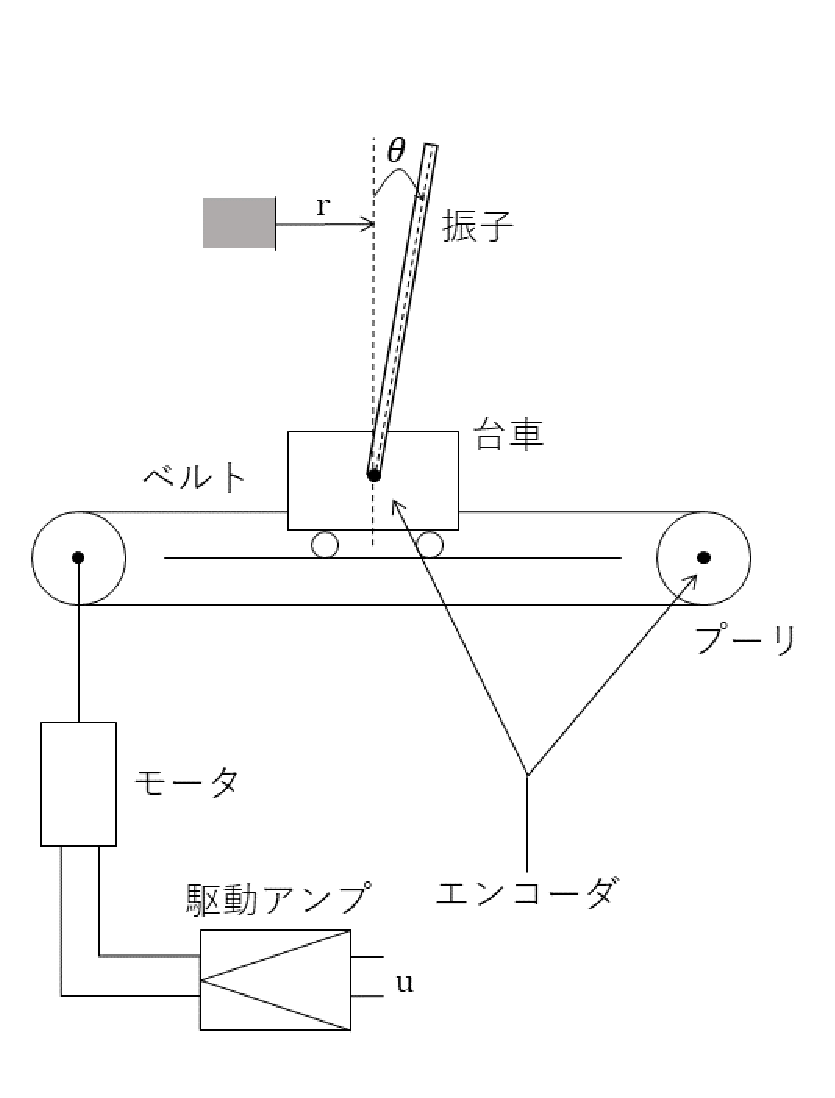
\includegraphics[width=0.8\linewidth]{gazo/pendulum.eps}
	\caption{倒立振子系}
	\label{image:pendulum}
\end{figure}
\begin{figure}[H]
	\centering
	\includegraphics[width=10cm,pagebox=cropbox,clip]{gazo/Pendulum.pdf}
	\caption{倒立振子系(写真)}
	\label{image:pendulum_photo}
\end{figure}
図\ref{image:pendulum}は倒立振子系を表す図である。モノレールの上に台車が置かれ、台車上のモノレールと直角な軸に1本の棒が取り付けられ、棒はその軸まわりに自由に回転できる。台車はベルトとプーリを介して、モータにより駆動され、
モノレール上を走行できる。すなわち、棒(振子)は鉛直線とモノレールにより定まる平面に拘束されて、台車によって動かされるようになっている\cite{Koga:Binpe}。
\par
図\ref{image:pendulum_photo}は実機の倒立振子である。駆動アンプは写っていないが、それ以外の部品は図\ref{image:pendulum}と同じように確認できる。この倒立振子系は机に固定されているわけではなく、
机の上に置かれているだけである。
\subsection{観測出力と操作入力}
倒立振子系の観測出力として、エンコーダにより、つぎの2つが測定できる。\\
\begin{itemize}
  \item 台車の基準位置から変位$r$に比例する電圧$y_{1}$
  \item 棒の鉛直線となす角度$\theta$に比例する電圧$y_{2}$
\end{itemize}
一方、操作入力は、つぎのものである。
\begin{itemize}
  \item モータの駆動アンプの入力電圧$u$
\end{itemize}
ここで、モータにより駆動される台車には、$u$に比例した駆動力が働くものとする\cite{Koga:Binpe}。
また、入力電圧の限界値は$-15<u<15$である。
%一次チェック完了:
%--------------------------------------------------------------------------------------------------------------


